The default settings for the experiments in this research are shown in table \ref{tab:default}. Preliminary results revealed the opponent color space in combination with dense SIFT outperforms the other methods and this combination is therefore chosen as default setting.

\begin{table}[H]
\begin{tabular}{|l|l|}
\hline
\textbf{Parameter} & \textbf{Default value}\\
\hline
Color space & Opponent\\
SIFT type & Dense\\
Training set size feature histogram & 75 per class\\
Training set size SVM & 75 per class\\
Test set size & 50 per class \\
Cluster size & 400 \\
Kernel & Sigmoid \\
Step size (only for dense SIFT) & 20\\
\hline
\end{tabular}
\caption{Default values for experiments}
\label{tab:default}
\end{table}
Linear kernel: $K(x,y) = (x+y)$\\
Polynomial kernel: $K(x,y) = (x^Ty + c)^d$\\
Sigmoid kernel: $K(x,y) = \text{tanh}(ax^Ty + r)$\\
Radial kernel: $K(x,y) = \text{exp}(-\frac{||x-y||^2}{s\sigma^2})$\\

Linear kernel is less complex, so less overfitting on noise. 

\subsection{Color spaces and SIFT methods}
As can be seen in table \ref{tab:key}, the normalized RGB color space shows the best results for automated image classification in comparison with the other color spaces when key-point SIFT is used. This result can be contributed to the fact that this color space is scale-invariant and invariant to light intensity changes. The opponent color space is also shift-invariant with respect to light intensity and shows a similar, but slightly lower, performance as the normalized RGB color space.  As the images of the dataset are mostly captured from the same point of view and have similar scales, the scale-invariance feature of the normalized RGB only slightly contributes to the automated image classification. The gray and RGB color spaces do not exhibit invariant features and therefore perform worse than the opponent and normalized RGB color spaces. These results are consistent with results from previous research by Sande et al.\cite{van2010evaluating}


\begin{table}[H]
\begin{tabular}{|c|ccccc|}
\hline
\textbf{Color space} & \textbf{AP Airplanes} & \textbf{AP Cars} & \textbf{AP Faces} & \textbf{AP Motorbikes} & \textbf{MAP}\\
\hline
gray & 0.8564 & 0.7468 & 0.6014 & 0.8485 & 0.7633\\
normalizedRGB & 0.9245 & 0.8081 & 0.8906 & 0.8308 & 0.8635 \\
RGB & 0.8870 & 0.8407 & 0.6821 & 0.8815 & 0.8228 \\
opponent & 0.8918 & 0.7946 & 0.8918 & 0.8457 & 0.8560\\
\hline
\end{tabular}
\caption{Effect of different color spaces for key SIFT}
\label{tab:key}
\end{table}

Table \ref{tab:color_sift} displays the results of different color spaces in use for dense SIFT. In contrast to the key-point SIFT method, the opponent color space gives the highest Mean Average Precision score for the dense SIFT method.  Surprisingly, normalized RGB color space obtains the lowest Mean Average Precision score for dense SIFT and is in contrast with the results of normalized RGB color for key-point SIFT. Because the default parameters for the window sizes are set small (4 and 8 pixels), features are extracted from small areas and more local features are extracted. The normalization of RGB possibly discards more distinctive local features than the other color space SIFT methods and therefore performs worse.\\

\begin{table}[H]
\begin{tabular}{|c|ccccc|}
\hline
\textbf{Color space} & \textbf{AP Airplanes} & \textbf{AP Cars} & \textbf{AP Faces} & \textbf{AP Motorbikes} & \textbf{MAP}\\
\hline
gray & 0.6476 & 0.7741 & 0.4292 & 0.8165 & 0.6668\\
normalizedRGB & 0.5743 & 0.3402 & 0.4678 & 0.5646 & 0.4867\\
RGB & 0.6424 & 0.9726 &  0.8689 & 0.6747 & 0.7897\\
opponent & 0.6447 & 0.9053 & 0.9510 & 0.7516 & 0.8132\\
\hline
\end{tabular}
\caption{Effect of different color spaces for dense SIFT}
\label{tab:color_sift}
\end{table}



\subsection{Effect number of training samples for feature histogram}
The effect of the number of training samples used for the creation of feature histograms is displayed in table \ref{tab:size_hist}. The results show that the Mean Average Precision increases when more training samples per class are used. This is because the visual vocabulary is formed with feature histograms which are more generalizing and thus the image features are more descriptive for each classifier. 
\begin{figure}[H]
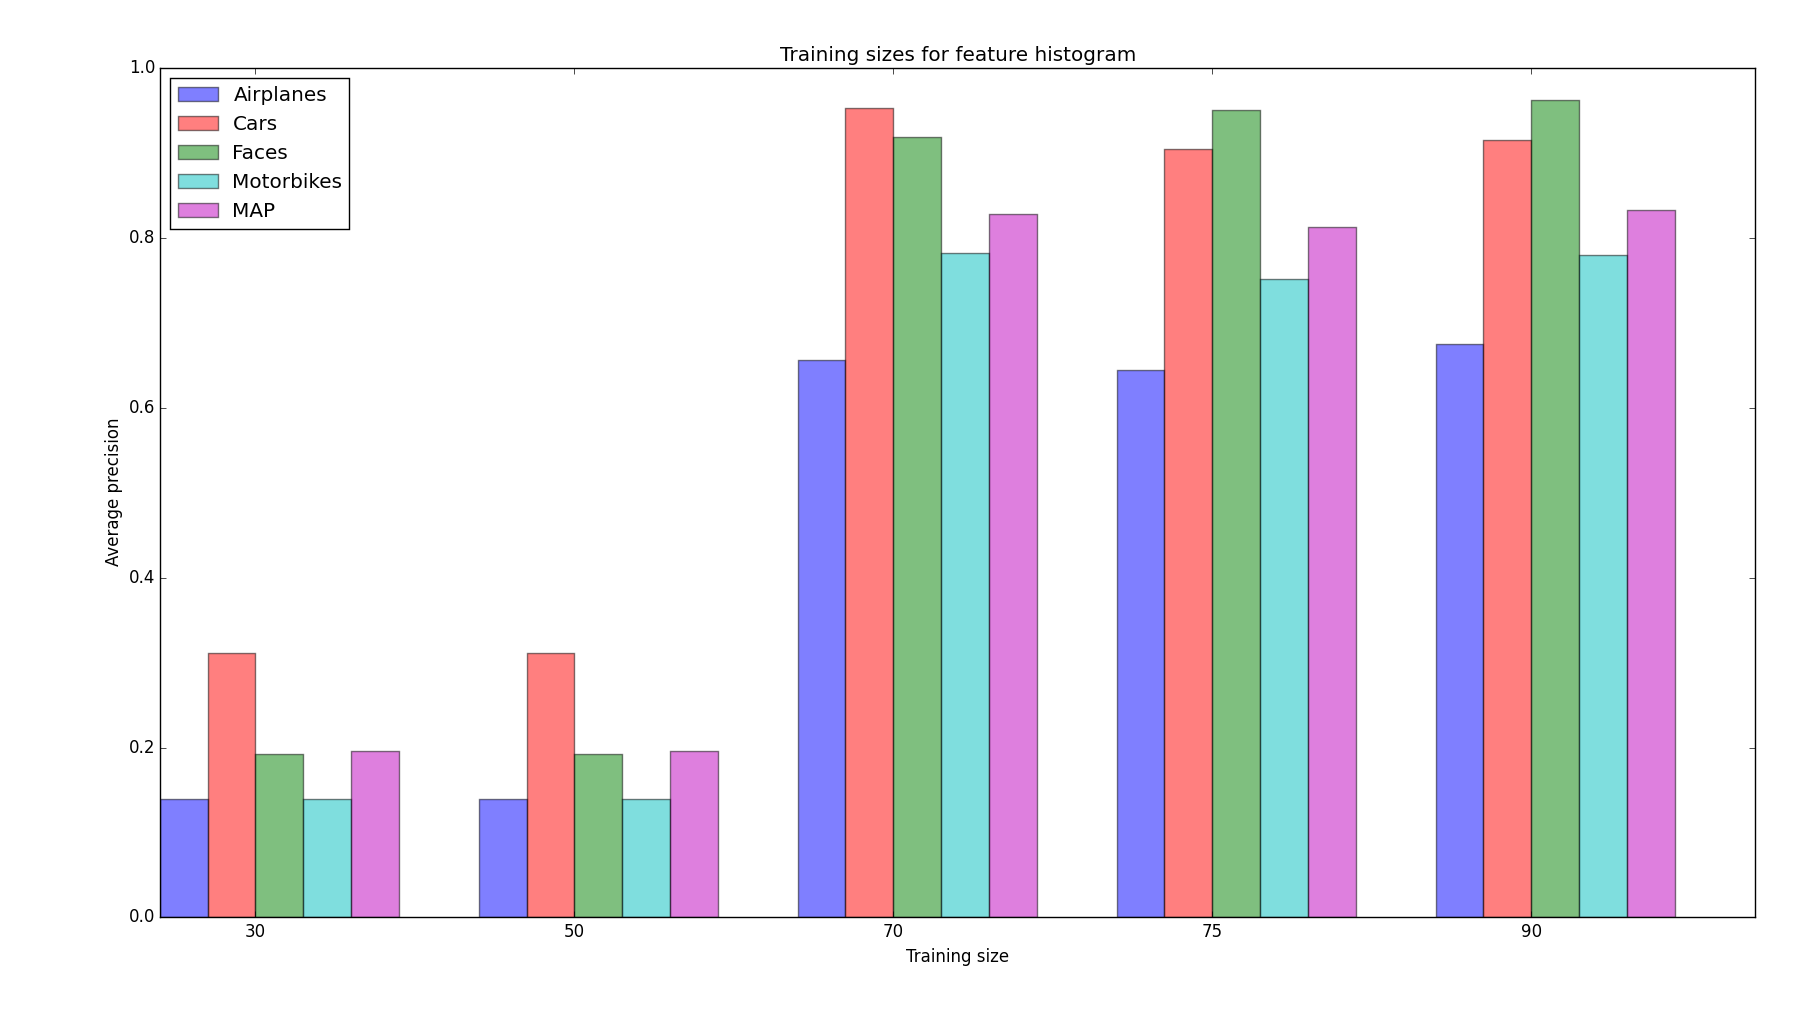
\includegraphics[width=\textwidth]{../plots/training_size_feature_histograms}
\caption{Effect of training size for histograms on AP}
\label{fig:size_hist}
\end{figure}
Figure \ref{fig:size_hist} shows clearly that the performance of the automated image classification stabilizes as the training samples size reaches approximately 70 images per class. This training sample size is sufficient for the generalization of feature histograms and enlarging the training sample size will not increase performance significantly. 

\begin{table}[H]
\begin{tabular}{|c|ccccc|}
\hline
\textbf{Training samples} & \textbf{AP Airplanes} & \textbf{AP Cars} & \textbf{AP Faces} & \textbf{AP Motorbikes} & \textbf{MAP}\\
\hline
30 & 0.1394 & 0.3118& 0.1924& 0.1394 & 0.1958\\
50 & 0.1394 & 0.3118& 0.1924& 0.1394 & 0.1958\\
55 & 0.6516 & 0.8392 & 0.6716 & 0.7797 & 0.7355\\
60 & 0.6535 & 0.8440 & 0.9905 & 0.2919 & 0.6950\\
65 & 0.6711 & 0.9483 & 0.9440 & 0.7688 & 0.8331\\
70 & 0.6563 & 0.9534 & 0.9191 & 0.7830 & 0.8280\\
75 & 0.6447 & 0.9053 & 0.9510 & 0.7516 & 0.8132\\
90 & 0.6749 & 0.9157 & 0.9631 & 0.7798 & 0.8334\\
\hline
\end{tabular}
\caption{Effect number of training samples (per class) for feature histogram, Sift type: dense, Color space: opponent}
\label{tab:size_hist}
\end{table}




\subsection{Effect number of training samples for SVM}

\begin{figure}[H]
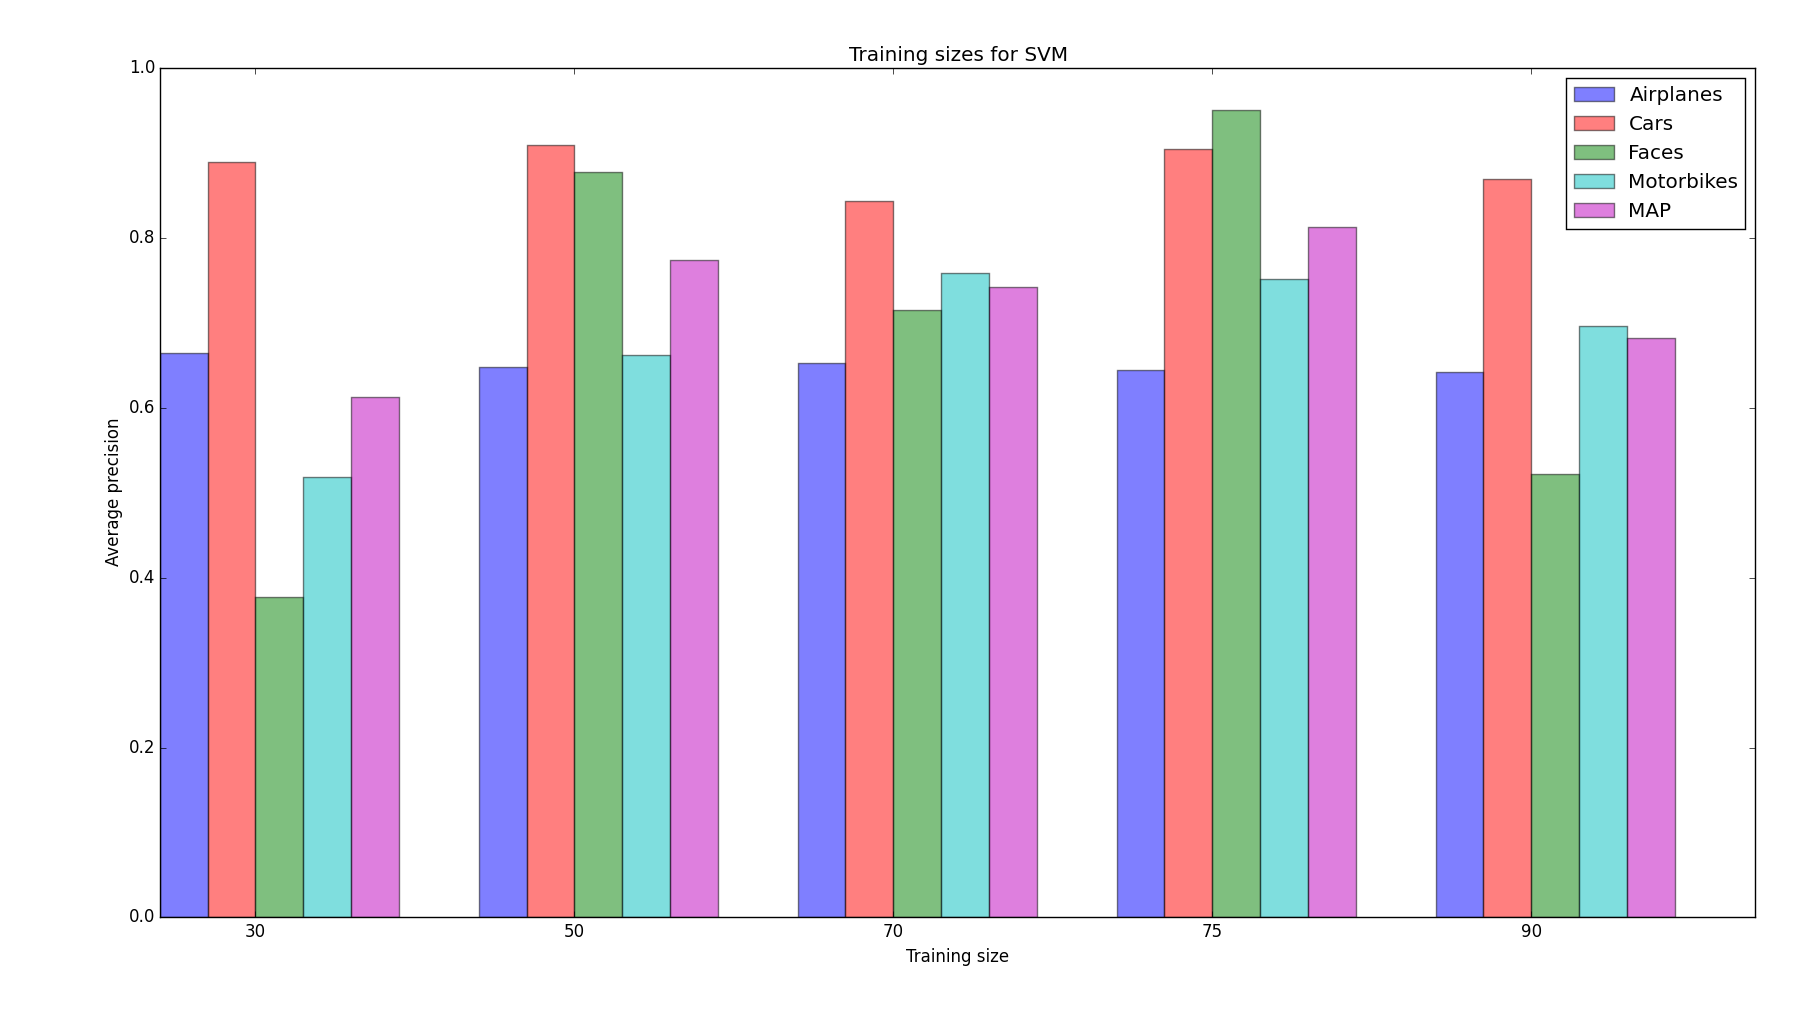
\includegraphics[width=\textwidth]{../plots/training_size_SVM}
\caption{Effect of training size for SVMs on AP}
\end{figure}

\begin{table}[H]
\begin{tabular}{|c|ccccc|}
\hline
\textbf{Training samples} & \textbf{AP Airplanes} & \textbf{AP Cars} & \textbf{AP Faces} & \textbf{AP Motorbikes} & \textbf{MAP}\\
\hline
30 & 0.6647 & 0.8898 & 0.3772 & 0.5184& 0.6125\\
50 & 0.6484 & 0.9096 & 0.8780 & 0.6627 & 0.7747\\
70 & 0.6531 & 0.8441 & 0.7156 & 0.7590 & 0.7429\\
75 & 0.6447 & 0.9053 & 0.9510 & 0.7516 & 0.8132\\
90 & 0.6426 & 0.8697 & 0.5227 & 0.6963 & 0.6828\\
\hline
\end{tabular}
\caption{Effect number of training samples (per class) for SVM, Sift type: dense, Color space: opponent}
\end{table}


\subsection{Effect of different cluster sizes}

\begin{figure}[H]
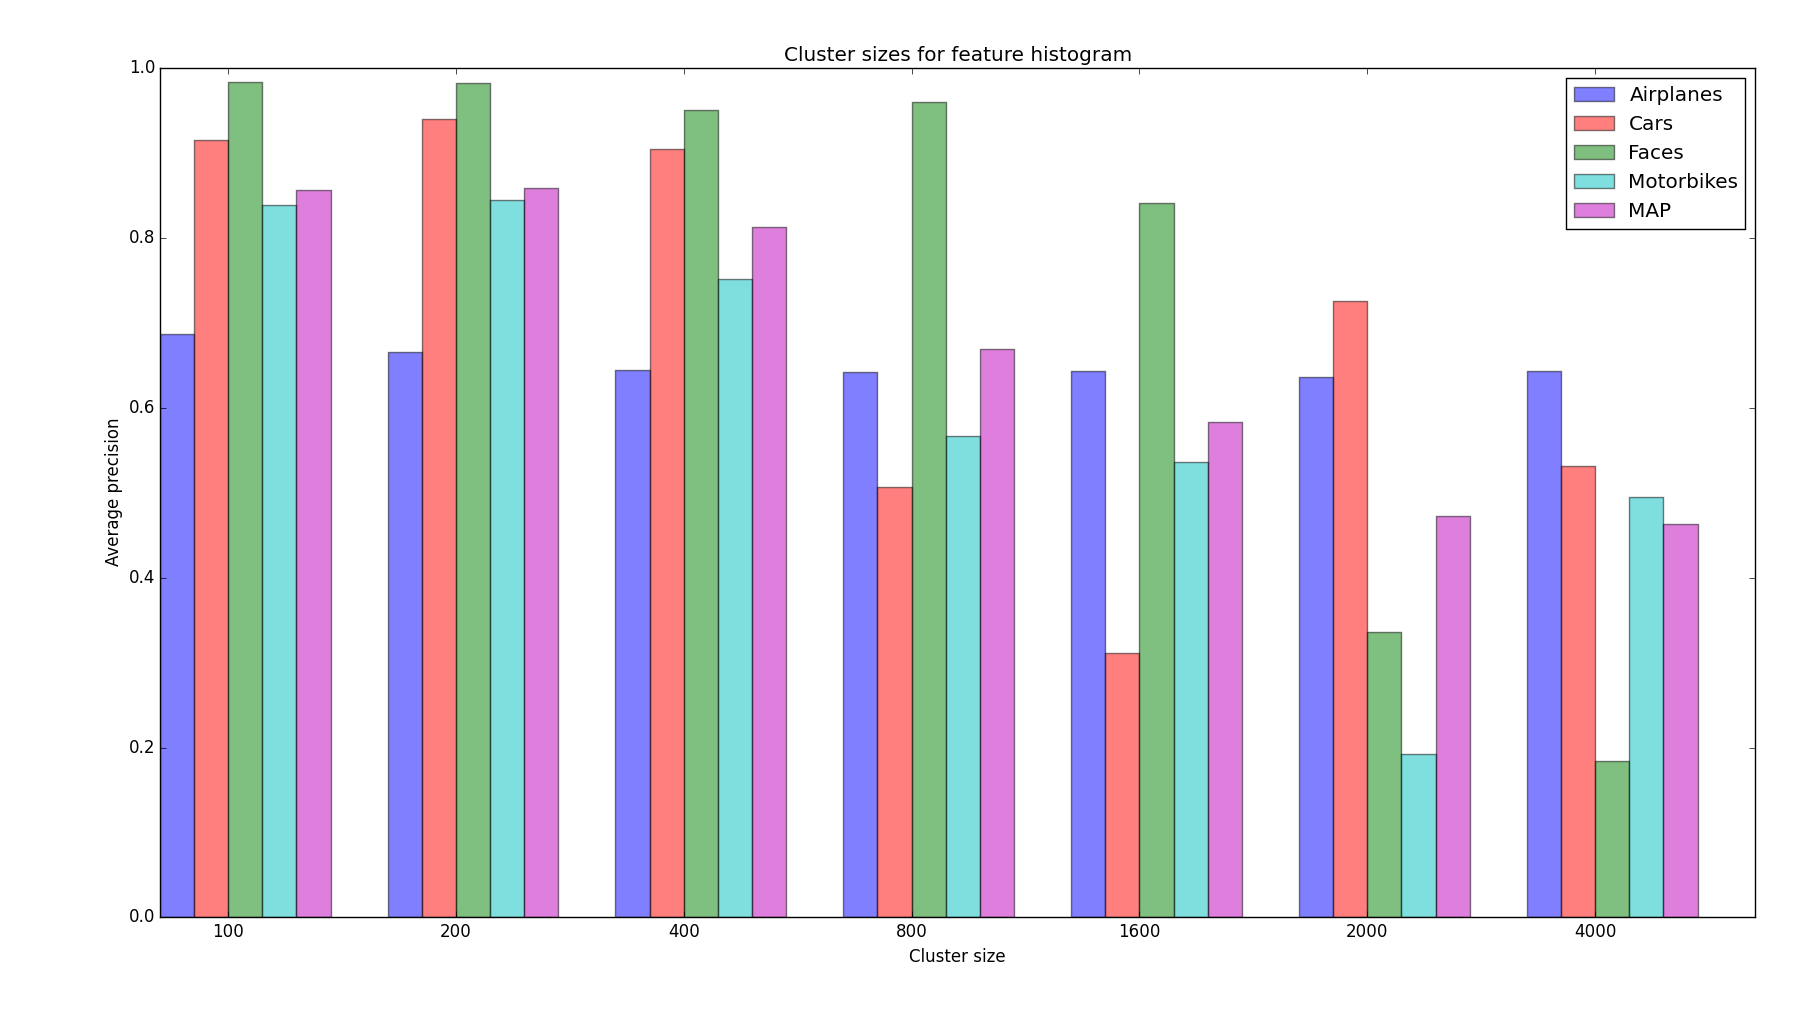
\includegraphics[width=\textwidth]{../plots/cluster_size_feature_histograms}
\caption{Effect of cluster size on AP}
\end{figure}
\begin{table}[H]
\begin{tabular}{|c|ccccc|}
\hline
\textbf{Cluster size} & \textbf{AP Airplanes} & \textbf{AP Cars} & \textbf{AP Faces} & \textbf{AP Motorbikes} & \textbf{MAP}\\
\hline
100& 0.6868 & 0.9152 & 0.9843 & 0.8395 & 0.8564\\
200 & 0.6663 & 0.9408 & 0.9824 & 0.8454 & 0.8587\\
400 & 0.6447 & 0.9053 & 0.9510 & 0.7516 & 0.8132\\
800 & 0.6424 & 0.5067 & 0.9602 & 0.5667 & 0.6690\\
1600 & 0.6438 & 0.3115 & 0.8410 & 0.5361 & 0.5831\\
2000 & 0.6367 & 0.7253 & 0.3357 & 0.1926 & 0.4726\\
4000 & 0.6430 & 0.5311 & 0.1837 & 0.4956 & 0.4634\\
\hline
\end{tabular}
\caption{Effect of different cluster sizes, Sift type: dense, Color space: opponent}
\end{table}

smaller cluster size is better: 200 still better dan 100. higher is probably overfitting, while 100 fails to capture enough features to differentiate between the different classes

\subsection{Effect of different step sizes for dense SIFT}
The effect of changing the step sizes for dense SIFT sampling can be seen in table \ref{tab:stepsize} and figure \ref{plot:stepsize}. A small step size, e.g. 10, underperforms compared to a slightly larger step size. However, when the step size is increased even more, the mean average precision of the algorithm rapidly decreases. The tipping point for the step size occurs at 20. This is due to a small step size resulting in a too detail oriented feature extraction, resulting in much noise and a tendency to overfit the data, while a large step size skips many details and tends to underfit the data. 

\begin{figure}[H]
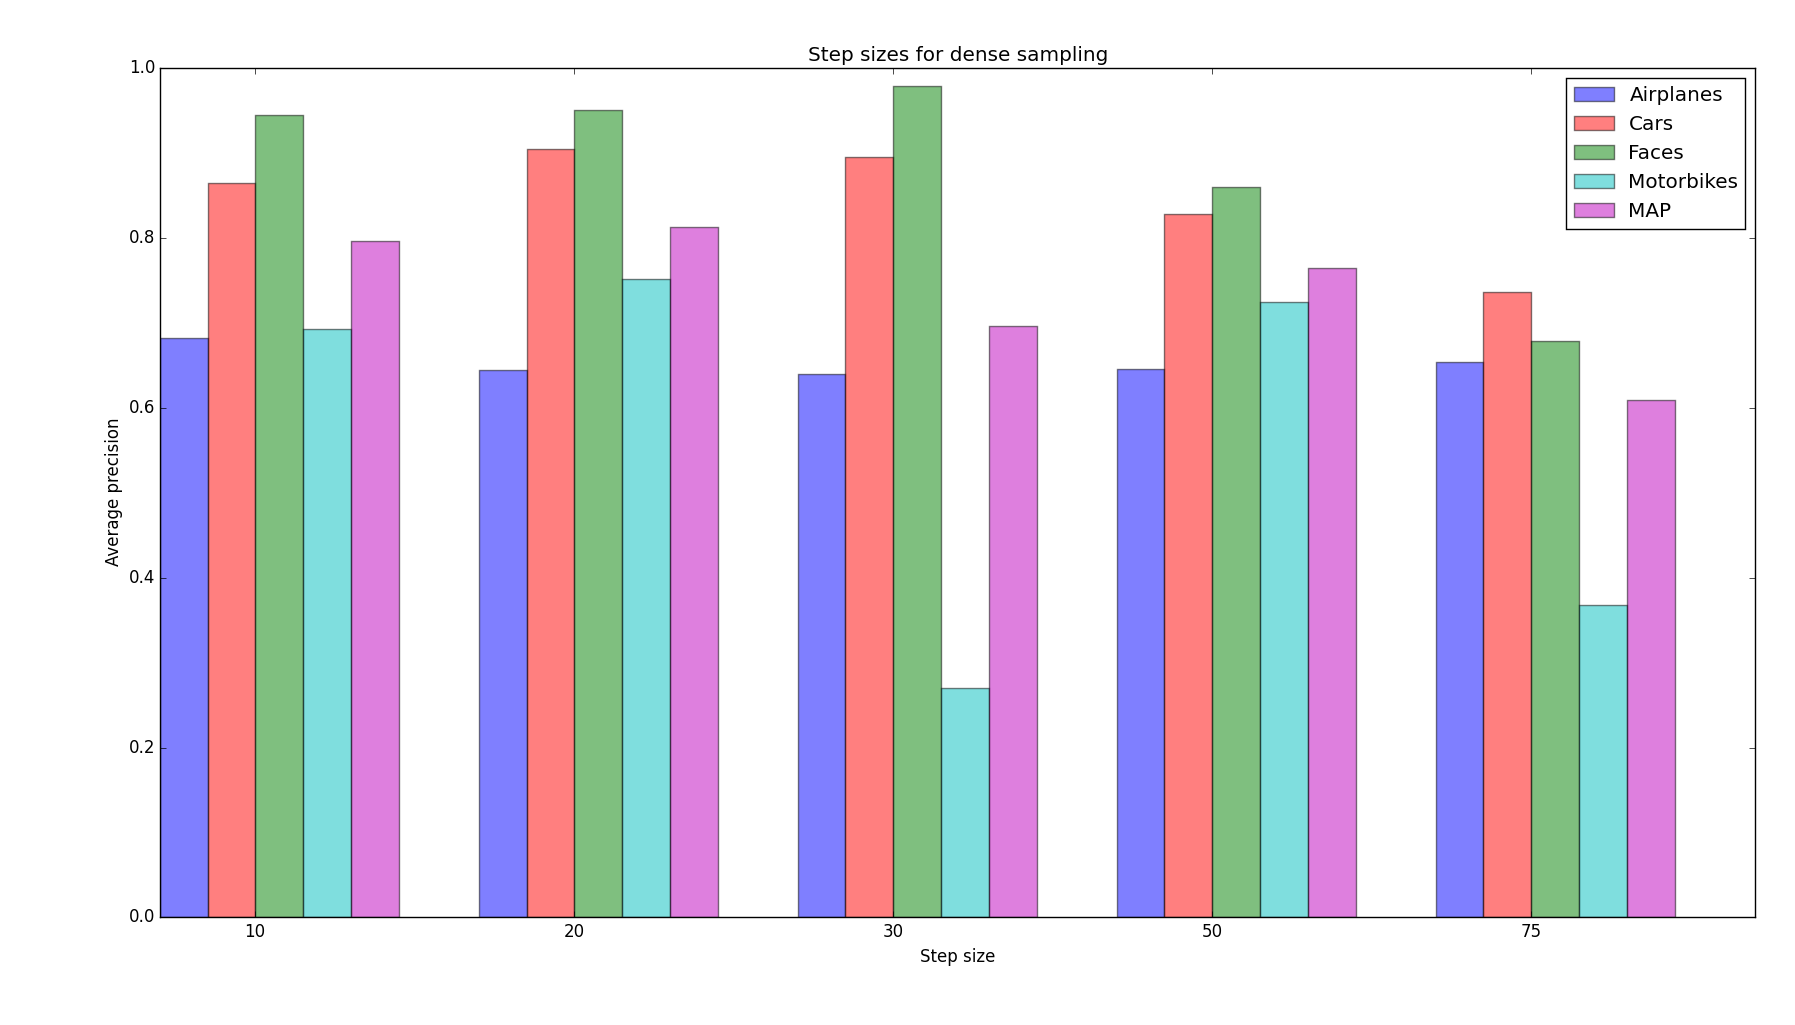
\includegraphics[width=\textwidth]{../plots/step_sizes_dense_sampling}
\caption{Effect of step size on AP}
\label{plot:stepsize}
\end{figure}
\begin{table}[H]
\begin{tabular}{|c|ccccc|}
\hline
\textbf{Step size} & \textbf{AP Airplanes} & \textbf{AP Cars} & \textbf{AP Faces} & \textbf{AP Motorbikes} & \textbf{MAP}\\
\hline
10 & 0.6823 & 0.8654 & 0.9444 & 0.6934 & 0.7964\\
20 & 0.6447 & 0.9053 & 0.9510 & 0.7516 & 0.8132\\
30 & 0.6405 &  0.8952& 0.9792& 0.2704 & 0.6963\\
50 & 0.6463 & 0.8288 & 0.8596 & 0.7247 & 0.7648\\
75 & 0.6539 & 0.7360 & 0.6791 & 0.3673 & 0.6091\\
\hline
\end{tabular}
\caption{Effect of different step sizes for dense SIFT Color space: opponent}
\label{tab:stepsize}
\end{table}



\subsection{Effect of different window sizes for dense SIFT}
\begin{figure}[H]
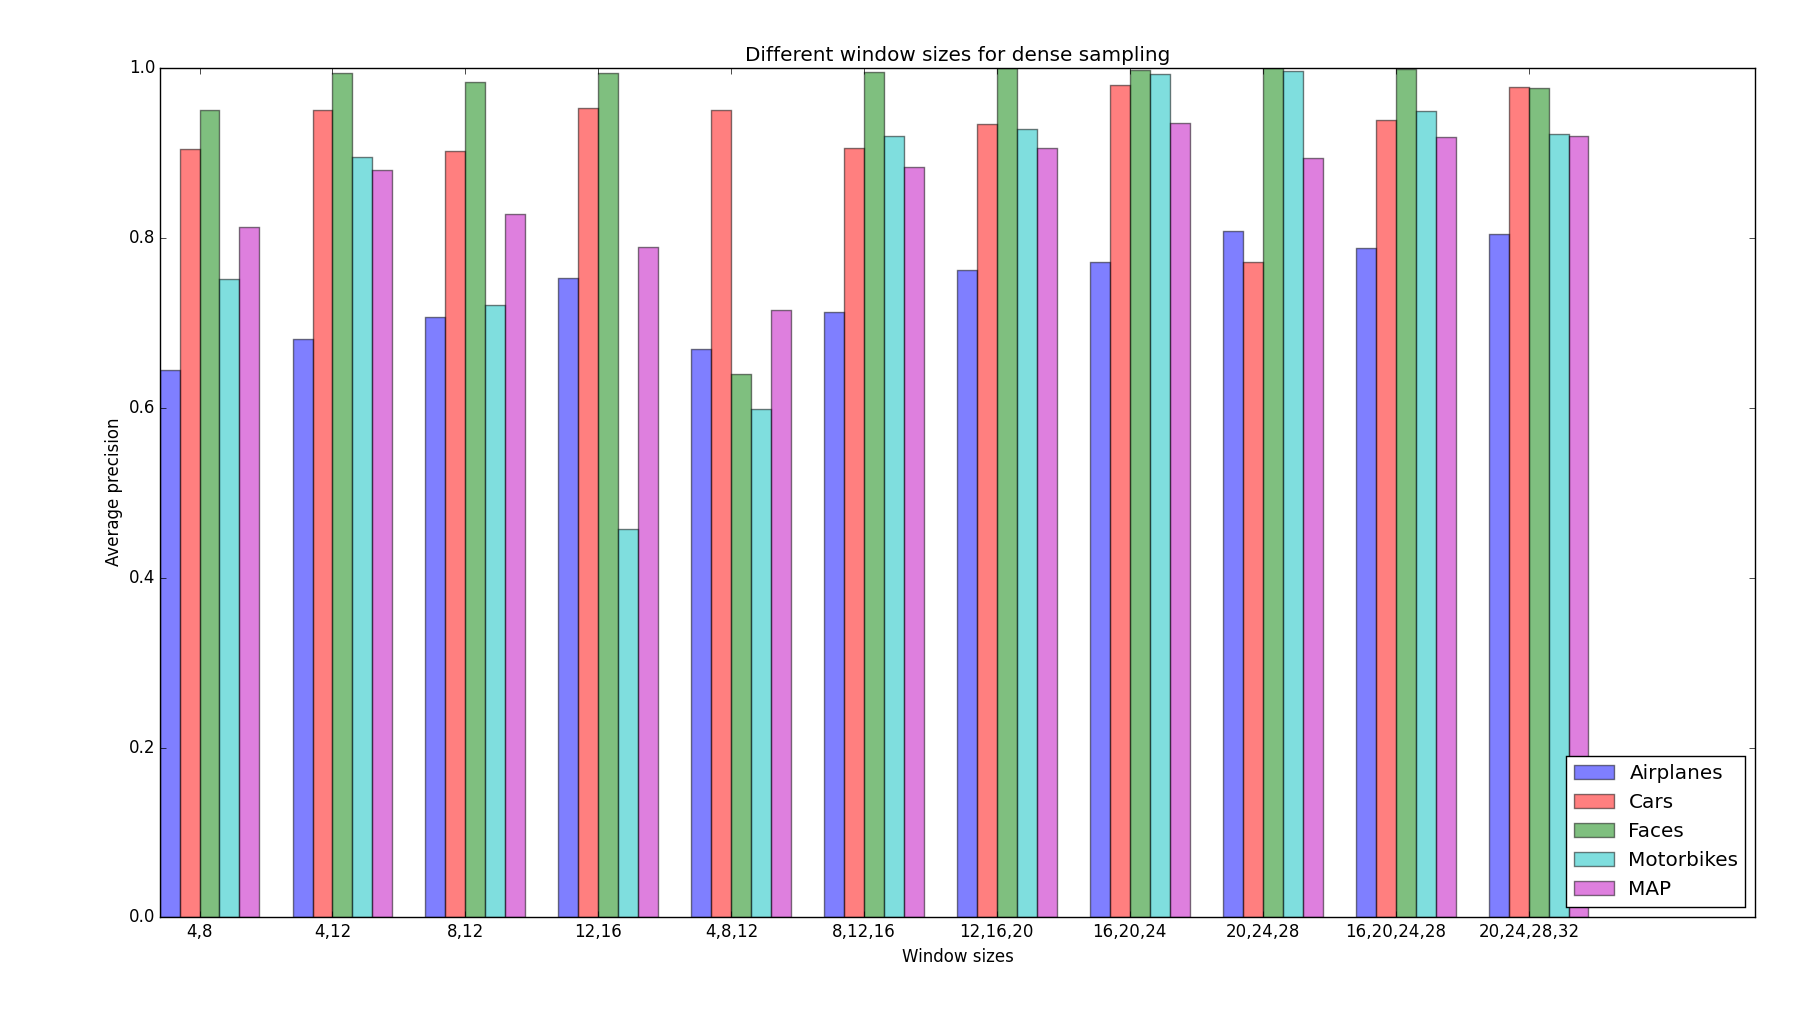
\includegraphics[width=\textwidth]{../plots/window_sizes_dense}
\caption{Effect of different window sizes on dense SIFT}
\end{figure}
\begin{table}[H]
\begin{tabular}{|c|ccccc|}
\hline
\textbf{Window size} & \textbf{AP Airplanes} & \textbf{AP Cars} & \textbf{AP Faces} & \textbf{AP Motorbikes} & \textbf{MAP}\\
\hline
4, 8 & 0.6447 & 0.9053 & 0.9510 & 0.7516 & 0.8132\\
4, 12 & 0.6809 & 0.9505 & 0.9945 & 0.8955 & 0.8803\\
8, 12 & 0.7066 & 0.9031 & 0.9839 & 0.7216 & 0.8288\\
12, 16 & 0.7532 & 0.9529 & 0.9939 & 0.4570 & 0.7893\\
4, 8, 12 & 0.6698 & 0.9511 & 0.6400 &  0.5987 & 0.7149\\
8, 12, 16 & 0.7133 & 0.9064 & 0.9952 & 0.9199 & 0.8837 \\
12, 16, 20 & 0.7629 & 0.9349 & 1.0000 & 0.9280 & 0.9065 \\
16, 20, 24 & 0.7719 & 0.9803 & 0.9981 & 0.9927 & 0.9357 \\
20, 24, 28 & 0.8086 & 0.7713 & 1.0000 & 0.9965 & 0.8941 \\
20, 24, 28, 32 & 0.8042 & 0.9782 & 0.9770 & 0.9223 & 0.9204 \\
16, 20, 24, 28 & 0.7882 & 0.9395 & 0.9989 & 0.9501 & 0.9192 \\

\hline
\end{tabular}
\caption{Effect of different window sizes for dense SIFT,  Color space: opponent}
\end{table}

BEST: 16,20,24
multiple window sizes capture a range of features, from details to larger features
Less gooder: 20,24,28,32 and 16,20,24,28: too many features, overfitting
less less gooder: 4,8 and 4,12 and 8,12 and 12,16 : small window sizes, can capture some details but not big enough to capture larger features (i.e. can capture eyes, wheels, but not wings and entire cars)

NEED TO TEST: 4,32 for example
also 4, 16, 32
also 4, 12, 24, 32




\subsection{Effect different kernels for SVM}

\begin{table}[H]
\begin{tabular}{|c|ccccc|}
\hline
\textbf{Kernel} & \textbf{AP Airplanes} & \textbf{AP Cars} & \textbf{AP Faces} & \textbf{AP Motorbikes} & \textbf{MAP}\\
\hline
sigmoid & 0.6447 & 0.9053 & 0.9510 & 0.7516 & 0.8132\\
linear & 0.6574 & 0.9668 & 0.9860 & 0.8642 & 0.8686 \\
polynomial & 0.7066 & 0.9031 & 0.9839& 0.7216& 0.8288\\
radial & 0.6491 & 0.9171 & 0.9438 & 0.7541 & 0.8160\\
\hline
\end{tabular}
\caption{Effect different kernels for SVM, Sift type: dense, Color space: opponent}
\end{table}
